\clearpage
\subsection{Workflow}\label{workflow}

In de website van \drupalpath wordt gebruik gemaakt van \emph{workflow}. Dat wil zeggen dat nieuwe inhoud en gewijzigde inhoud niet in alle gevallen direct op de site zal verschijnen, maar eerst goedgekeurd moet worden. Hierbij wordt onderscheid gemaakt tussen eindredacteuren en redacteuren. Eindredacteuren hebben het recht om content binnen de gehele website te publiceren en aan te passen. Eindredacteuren kunnen content van redacteuren tevens publiceren op andere delen van de site.

De workflow is zowel van toepassing op nieuwe als bestaande inhoud. Bij reeds bestaande inhoud wordt een nieuwe \emph{revisie} aangemaakt. De nieuwe revisie kan bestaan naast de gepubliceerde pagina. Zo is het mogelijk dat een wijziging pas later, na goedkeuring, gepubliceerd wordt en dus zichtbaar voor bezoekers.

Bij het invoeren of bewerken van content is onderin het formulier een item "Publicatie-opties" te zien. Hierin staat een item "Moderatie status". Daarin zitten de volgende opties:
\begin{itemize}
\item Mijn concepten
\item Te beoordelen
\item Gepubliceerd
\end{itemize}

Nieuwe inhoud of revisies worden als eerste aangemaakt als \emph{concept}. In deze staat is het een 'kladversie'. Bewerkingen hebben nog geen invloed op de website. Wanneer de content online mag dan kan de status op \emph{Te beoordelen} worden gezet. In deze staat krijgen eindredacteuren dit item te zien in een lijst met goed te keuren inhoud. Tevens wordt een mail gestuurd naar alle eindredacteuren. Het item kan daarna op \emph{Gepubliceerd} worden gezet. De inhoud wordt dan zichtbaar op de website voor alle bezoekers. Afhankelijk van de rechten is het mogelijk om in dit proces stappen over te slaan.


Onderstaand tabel toont de workflow per inhoudstype. 

\textbf{Gepubliceerd:} Na het opslaan wordt de content direct zichtbaar gemaakt op de website.

\textbf{Revisie:} Elke keer nadat een content item is bijgewerkt, wordt er een nieuwe revisie aangemaakt.

\textbf{Moderatie revisie:} Indien deze optie is geactiveerd, is het mogelijk een revisie te wijzigen.

\textbf{Ge{\"\i}mporteerd:} Content van dit inhoudstype zal ge{\"\i}mporteerd worden.

\textbf{J:} Ja (van toepassing).

\textbf{N:} Nee (niet van toepassing).

\begin{tabularx}{\textwidth}{ | p{5cm} |X|X|X|X| }
  \hline
  Inhoudstype & Gepubliceerd & Revisie & Moderatie revisie & Ge{\"\i}mporteerd \\ \hline
  Agenda & N & J  & J & N  \\ \hline
  Bekendmaking & N & J  & J & J  \\ \hline
  Bericht  & J & N  & N & N  \\ \hline
  Bestand  & J & N  & N & N  \\ \hline
  Bestemmingsplan  & J & N  & N & J  \\ \hline
  Blog  & J & N  & N & N  \\ \hline
  Editorial  & J & J  & N & N  \\ \hline
  Eenvoudige pagina  & N & J  & J & N  \\ \hline
  FAQ  & N & J  & J & N  \\ \hline
  Forumonderwerp  & J & N  & N & N  \\ \hline
  Foto  & J & N  & N & N  \\ \hline
  Marktplaats  & J & N  & N & N  \\ \hline
  Nieuws  & N & J  & J & N  \\ \hline
  Onderwerp  & J & N  & N & N  \\ \hline
  Peiling  & N & J  & J & N  \\ \hline
  Persoon  & N & J  & J & N  \\ \hline
  Product  & J & N  & N & J  \\ \hline
  RSS  & J & N  & N & J  \\ \hline
  RSS Source  & N & N  & N & N  \\ \hline
  Regeling  & J & N  & N & J  \\ \hline
  Slide  & N & J  & J & N  \\ \hline
  VAC  & J & N  & N & J  \\ \hline
  Webformulier  & J & N  & N & N  \\ \hline
  Wiki  & J & N  & N & N  \\ \hline
\end{tabularx}

\subsubsection{Revisies inzien en terugzetten}\label{modererentab}

De revisies van inhoud zijn later (ook na publicatie) terug te vinden onder het tabblad "Modereren". Op deze pagina is een lijst te zien waarin tevens de datum en workflow status te zien is. Met de link "weergeven" kan de revisie worden bekeken. Met de link "terugzetten" kan de revisie worden teruggezet. In het laatste geval publiceren we een oudere revisie, waarmee we alle latere wijzigingen ongedaan maken. Een revisie kan ook nieuwer zijn dan de versie die is gepubliceerd. In dit geval is er een "publiceren" link aanwezig. Hiermee kan deze versie worden goedgekeurd en gepubliceerd.

Onder de link "Vergelijk revisies" (2e niveau tabblad) zit een pagina waarmee makkeljik te verschillen tussen revisies zichtbaar gemaakt kunnen worden. Hierbij moeten twee revisies gekozen worden. Kies eerst de nieuwste revisie en daarna de oudere revisie (verder onderaan in de lijst). Klik daarna op de knop \emph{Vergelijken}. Hierna worden de tekstuele wijzigingen getoond. Dit heeft betrekking op de hoofdtekst van dit item.

\subsubsection{Inhoud goedkeuren}\label{inhoudgoedkeuren}

In het dashboard is voor eindredacteuren een lijst beschikbaar met inhoud dat goedgekeurd dient te worden. Dit is inhoud met de status \emph{Ter beoordeling}. Klik hiervoor linksboven op "Mijn Workbench" en dan op "Te beoordelen" (2e niveau tabblad). In deze lijst kan doorgeklikt worden naar de pagina's die goedgekeurd dienen te worden. Nadat de wijzigingen zijn bekeken kunnen deze worden goedgekeurd onder het tabblad "Modereren"\seeone{modererentab}.

\begin{center}
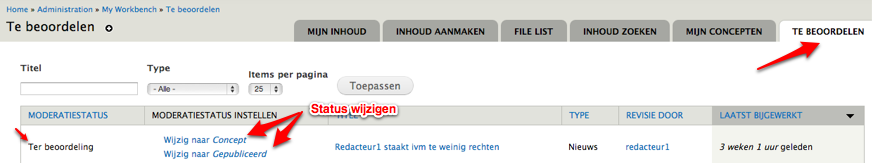
\includegraphics[width=\textwidth]{img/publiceren.png}
\end{center}